\paragraph{4. Do the lost relations result in New Observable Behaviors?}

    To address this, we divide our cases into two parts; one for each type of relation lost:
    \begin{tasks}(2)
        \task $\reln{k}{hb}{W_{uo}}$
        \task $\reln{W_{uo}}{hb}{k}$
    \end{tasks}

    Figure~\ref{elim_write:case1} shows a breakdown of sub-cases for case (a), varying based
    on the nature of event $k$.
    \begin{figure}[H]
        \centering
        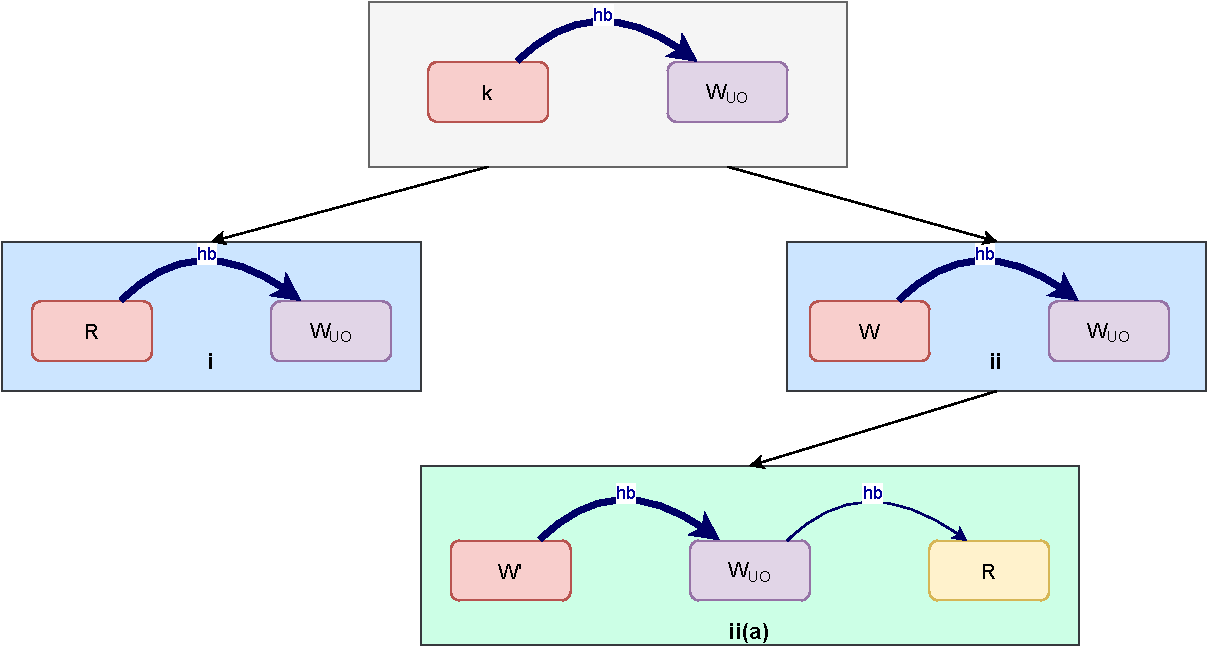
\includegraphics[scale=0.5]{6.Elimination/1.ValidEliminationCandidate/WriteElimProof/ProofParts/Part4Case1.pdf}
        \caption{The impact of lost relation $\reln{k}{hb}{W_{uo}}$ on observable behaviors.}
        \label{elim_write:case1}
    \end{figure}

    We can observe the following:
    \begin{itemize}
        \item (i) is a pattern from Axiom \ref{CoRe} that restricts the read $R$ reading from $e$. This will remain the case even after elimination of $e$.
        \item (ii)(a) is a pattern from Axiom \ref{CoRe}, forbidding $R$ to read some bytes of $W'$. 
        This will remain the case after elimination of $e$ if firstly we have $\reln{d}{hb}{R}$ and $\reln{W}{hb}{d}$.
        By Lemma \ref{Lemma2}, the first relation holds and by Def of happens-before the second holds. 
        Secondly, we need to ensure that after elimination, Axiom \ref{CoRe} now restricts the exact set of $\stck{_{rbf}}$ relations with $W'$ and $R$ as before. 
        Since $R$ or $W'$ can be arbitary, we would need the ranges of $e$ and $d$ to be same.
    \end{itemize}

    Figure~\ref{elim_write:case2} shows a breakdown of sub-cases for case (b), varying based
    on the nature of event $k$.
    \begin{figure}[H]
        \centering
        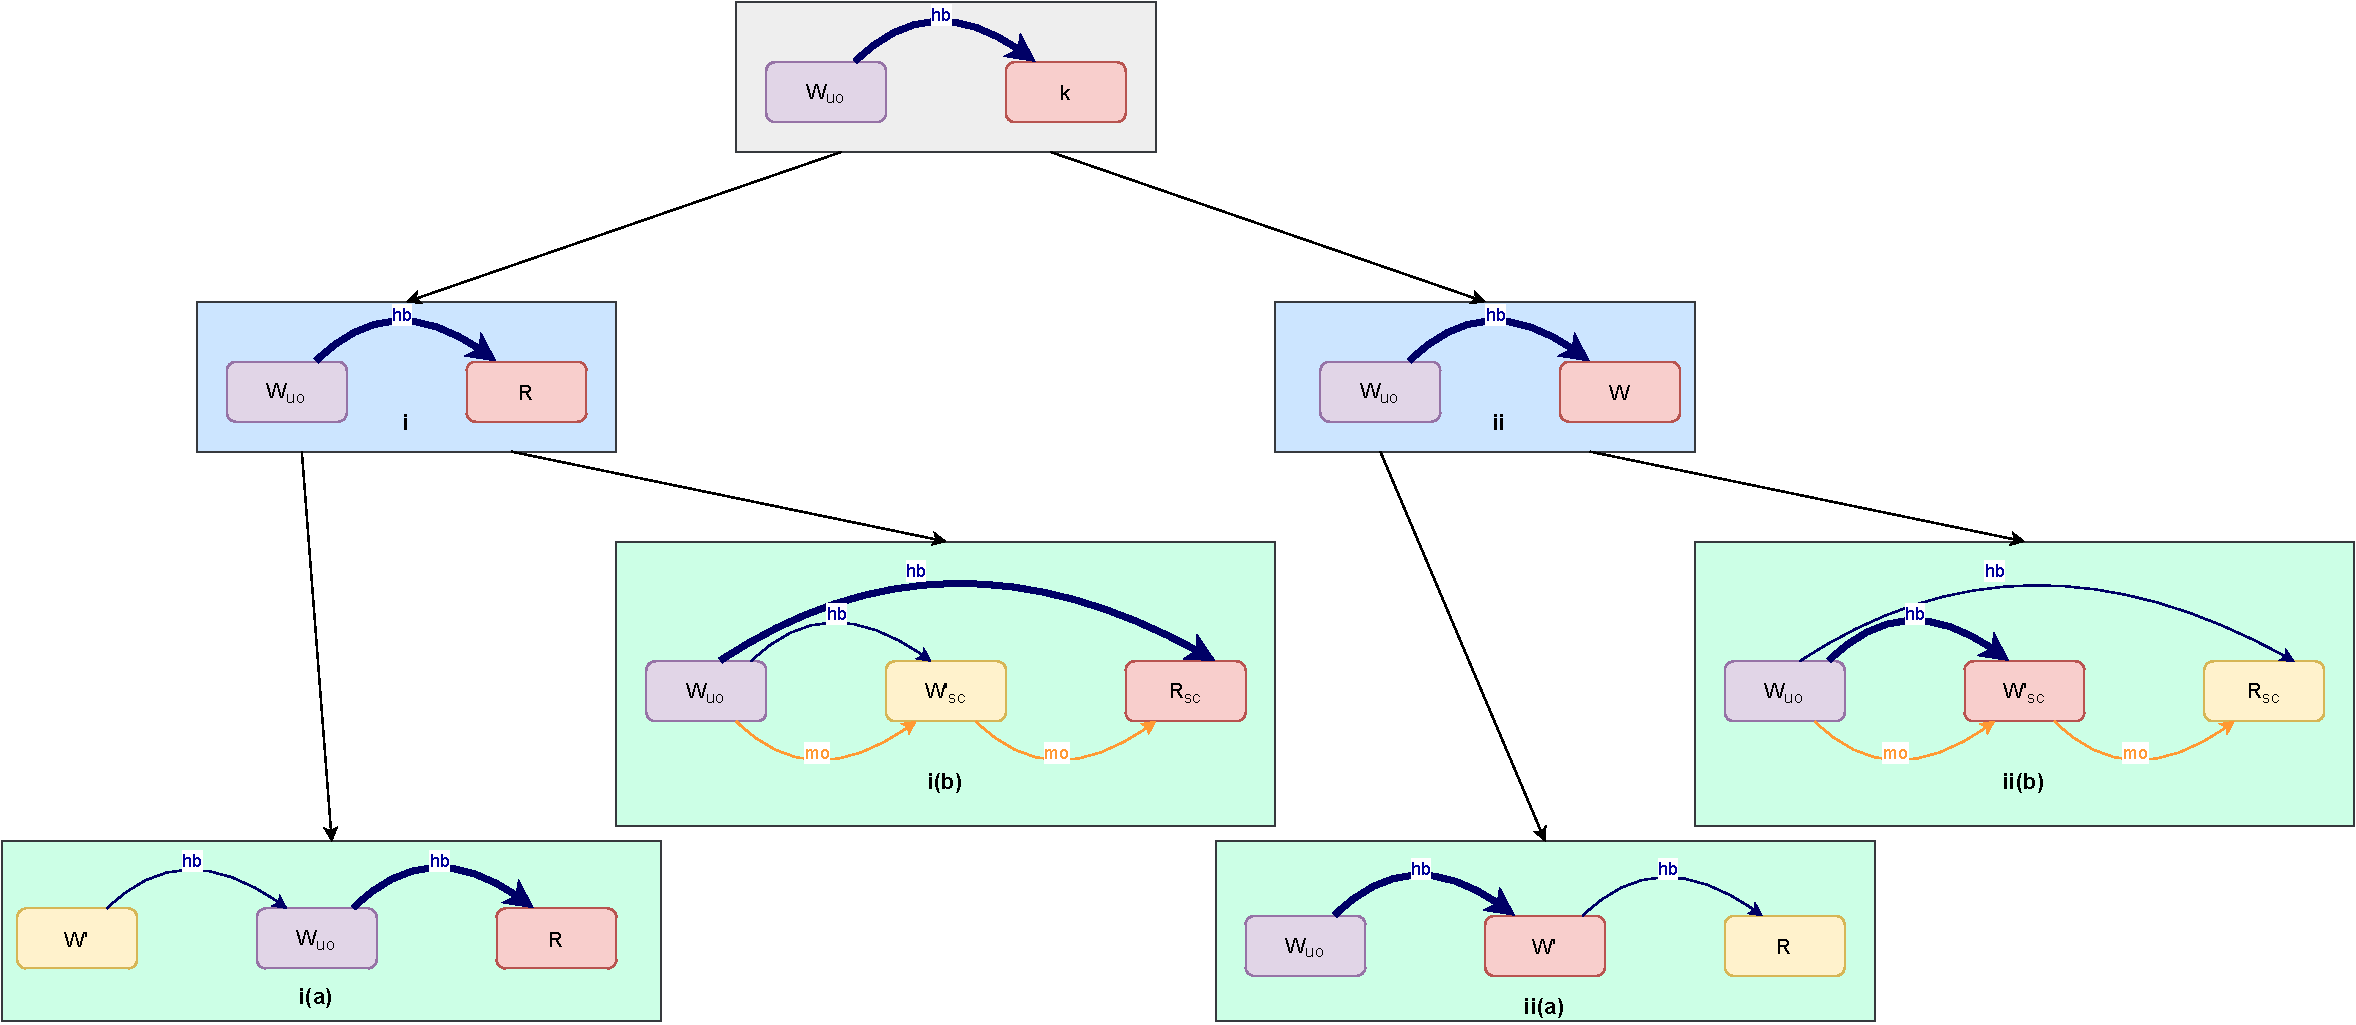
\includegraphics[scale=0.3]{6.Elimination/1.ValidEliminationCandidate/WriteElimProof/ProofParts/Part4Case2.pdf}
        \caption{The impact of lost relation $\reln{W_{uo}}{hb}{k}$ on observable behaviors.}
        \label{elim_write:case1}
    \end{figure}

    We make the following observations:
    \begin{itemize}
        \item (i)(a) has the similar argument to the previous case's (ii)(a), requiring $e$ and $d$ to have equal ranges.
        \item (i)(b) is a pattern from Axiom \ref{SeqCsAt}, which restricts $R$ from reading anything of $W$. This will reamin the case after $W$ is eliminated. 
        \item (ii)(a) is a pattern from Axiom \ref{CoRe}, restricting $R$ from reading $W$. This will remain the case after eliminating $W$.
        \item (ii)(b) is the same as (i)(b), hence the argument remains the same.  
    \end{itemize}

    In all the above cases, observe that on keeping range of $e$ and $d$ equal, none of the patterns introduce any new observable behavior. Hence, if we have two consecutive writes of equal ranges, of which the first one has access mode unorderd, the set of Observable Behaviors without the write is a subset of that with it present. 

    \critic{purple}{This can be slightly modified to show that the range of $e$ can even just be contained in $d$. This would ensure we can eliminate writes in more other cases.}